\documentclass[10pt,letterpaper]{article}
\usepackage[T1]{fontenc}
\usepackage{times,microtype,graphicx,booktabs,float}
\usepackage[font=small,labelfont=bf,labelsep=period,skip=4pt]{caption}
\setlength{\textwidth}{6in}
\setlength{\textheight}{9in}
\setlength{\oddsidemargin}{0.25in}
\setlength{\evensidemargin}{0.25in}
\setlength{\topmargin}{-0.35in}
\setlength{\headheight}{0.15in}
\setlength{\headsep}{0.2in}
\setlength{\parindent}{0pt}
\setlength{\parskip}{4pt}
\setlength{\intextsep}{4pt}
\setlength{\textfloatsep}{9pt}
\newcommand{\reporttitle}[2]{\noindent\rule{\linewidth}{4pt}\par
{\LARGE\bfseries #1\par}\vspace{2pt}\noindent\rule{\linewidth}{1pt}\par
#2\par October 16, 2026\par\vspace{4pt}}
\makeatletter
\renewcommand\section{\@startsection{section}{1}{\z@}{9pt}{4pt}{\large\bfseries}}
\makeatother
\renewenvironment{abstract}{\small\textbf{Abstract}\par}{\par\vspace{3pt}}
\let\originalitemize\itemize
\renewcommand{\itemize}{\originalitemize\setlength{\itemsep}{1pt}\setlength{\parskip}{0pt}\setlength{\parsep}{0pt}}
\let\originalenumerate\enumerate
\renewcommand{\enumerate}{\originalenumerate\setlength{\itemsep}{1pt}\setlength{\parskip}{0pt}\setlength{\parsep}{0pt}}
\begin{document}
\reporttitle{Reference and annotation comparison}{Arabidopsis TAIR10 and Col-CEN; fixed inputs and explicit coordinate mapping}
\begin{abstract}At 1 million ATAC pairs, reciprocal peak Jaccard is 0.8984 and 0.9639 between TAIR10 and Col-CEN for two replicates. A completed local 5-million-pair assessment gives 0.9547 and 0.9571 among eligible mappings. Annotation alone changes TSS scores on identical aligned reads, and mapping exclusions limit every cross-assembly claim. We would choose reference and annotation explicitly rather than rank them by peak count or TSS enrichment.\end{abstract}
\section*{Setup}
\textbf{Data.} The same paired ATAC subsets and both-mate MAPQ30 selection are used for each assembly, with duplicate and organellar exclusion. Each reference supplies its own effective genome size; peak calling therefore also reflects a changed background model.

\textbf{Scoring.} Reciprocal conversion requires at least 95\% aligned bases in each direction, unique placement and at least 95\% round-trip span overlap. Jaccard uses eligible peak-base unions in the destination assembly. Spearman compares fragment counts on baseline intervals and their eligible projections; widths may differ.

\begin{table}[H]\centering\small\caption{Input identities at the atac-arabidopsis-1m cap.}
\begin{tabular}{lrr}\toprule
Library & Role / control & Raw templates \\ \midrule
SRR4000468 & biological replicate 1 & 1,000,000 \\
SRR4000469 & biological replicate 2 & 1,000,000 \\
\bottomrule\end{tabular}\end{table}
\section{Eligible regions agree strongly across the two assemblies}
At 1 million pairs, matched-region Spearman is 0.9979 and 0.9946 for 4,992 and 3,040 eligible TAIR10 peaks. At 5 million pairs, it is 0.9990 and 0.9977; these are existing recorded results, not newly rerun analyses.

\begin{figure}[H]\centering\makebox[\linewidth][c]{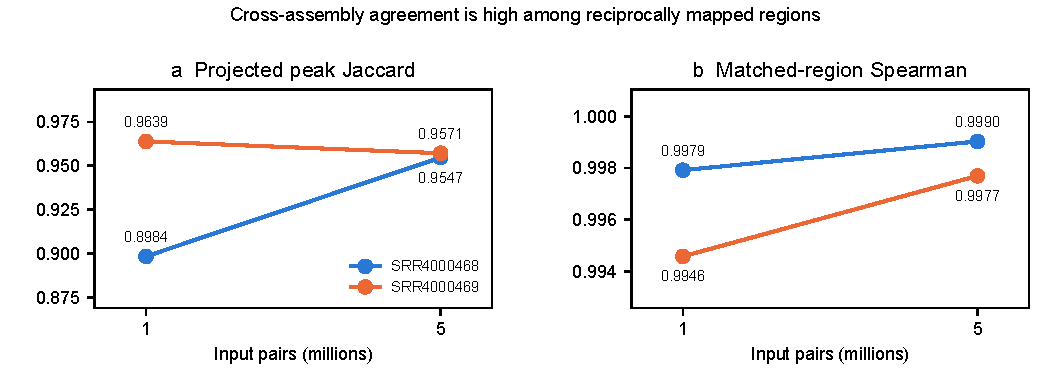
\includegraphics[width=7in]{figures/references.pdf}}
\caption{Reciprocal-coordinate agreement at two read depths.}\end{figure}
\newpage
\section{Coordinate exclusions remain part of the result}
\begin{table}[H]\centering\small\caption{Peak eligibility before cross-assembly comparison.}
\begin{tabular}{lrrr}\toprule
Million pairs & Library & TAIR10 accepted / total & Col-CEN accepted / total \\ \midrule
1 & SRR4000468 & 4,992 / 4,997 & 5,586 / 5,596 \\
1 & SRR4000469 & 3,040 / 3,043 & 2,968 / 2,977 \\
5 & SRR4000468 & 14,788 / 14,805 & 15,312 / 15,343 \\
5 & SRR4000469 & 11,538 / 11,551 & 11,905 / 11,930 \\
\bottomrule\end{tabular}\end{table}
At the 1-million-pair cap, 8 TAIR10 and 19 Col-CEN peaks across the 2 libraries fail the reciprocal criteria. Excluded, ambiguous or unmapped intervals are not assigned to a convenient first placement.

\textbf{Evidence revision.} The public October 14 snapshot described the 5-million-pair mapping as pending. Its later completed assessment now has a matching SHA-256 completion receipt. The accompanying compact audit preserves the result, mapping, script and experiment hashes; it does not overwrite the historical report or distribute the local BAMs.

\section{Reference distribution names do not guarantee new sequence}
The A. lyrata audit reports identical case-insensitive sequence multisets for 695 contigs totaling 206,667,935 bases in the Ensembl v1.0 and Phytozome v2.1 distributions. All 695 contigs have unique full-sequence matches, while names and order differ.

\begin{table}[H]\centering\small\caption{Reference preparation is distinct from a sequencing comparison.}
\begin{tabular}{p{1.35in}p{2.2in}p{1.85in}}\toprule
Comparison & Completed evidence & Not established \\ \midrule
A. lyrata distributions & 695 exact contig matches & Newer sequence improves peaks \\
Maize AGPv4 / NAM5 & 1,003 forward / 2,413 reverse chains checked & Sequencing method superiority \\
Sorghum assemblies & Reference acquisition records & Validated peak concordance \\
\bottomrule\end{tabular}\end{table}
\textbf{Limits.} Uniqueness is bounded by the supplied assembly alignments, not a proof that every repetitive placement is represented. Comparison within retained coordinates does not establish overall assembly accuracy, and neither reference has independent biological ground truth here.

\newpage
\section{Annotation changes TSS enrichment without changing reads}
On identical Col-CEN BAMs, all-start TSS sets contain 46,558 Araport and 32,986 TAIR positions. For replicate SRR4000469, the score is 2.7517 with Araport versus 3.2096 with TAIR; the common-gene comparison retains 18,428 eligible starts per annotation.

\begin{figure}[H]\centering\makebox[\linewidth][c]{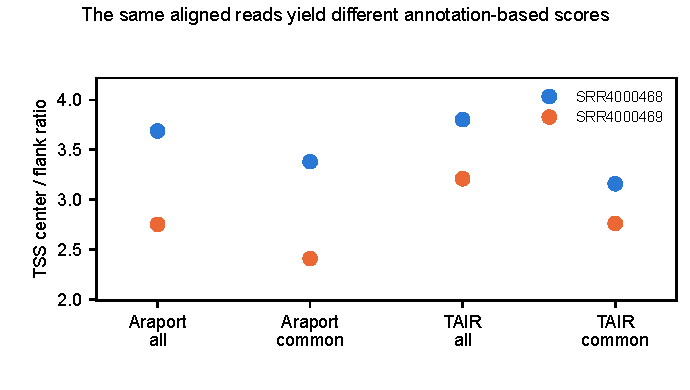
\includegraphics[width=4.6in]{figures/annotations.pdf}}
\caption{TSS enrichment with all-start and common-gene annotation sets.}\end{figure}
\textbf{Metric.} Tn5 cut positions use zero-based start+4 and end-6. The enrichment ratio divides the center bin by mean outer 100-base flanks across full 2,000-base windows on each side. Of 18,430 common single-start genes, 2 edge positions lack full windows; common genes can have different TSS positions across annotations.

\section*{Open issues}
\begin{itemize}
\item Higher TSS enrichment does not prove better annotation or library quality.
\item Matched-coordinate agreement excludes precisely some difficult assembly regions.
\item The broader species sequencing panel is not established by reference acquisition alone.
\end{itemize}
\section*{Recommendation}
We would record sequence identity and annotation suitability as separate decisions.

\begin{enumerate}
\item Choose the assembly and gene models required by the intended downstream task.
\item Retain coordinate exclusions and compare independent regulatory evidence.
\end{enumerate}
\section*{Appendix: Methods}
We summarize recorded results without rerunning biological processing. The main Arabidopsis matrix uses seeded nested raw-template subsets (seed 60141), three fresh technical repetitions at the 1-million cap and one at the 5-million cap. Actual counts replace requested caps for short libraries. DAP retains primary mapped reads including MAPQ 0; ATAC selects proper primary pairs with both mates MAPQ at least 30, excludes MAPQ 255, organelles and marked duplicates. Biological identity is preserved. Source files are SHA-256 checked against the accompanying catalog; evidence snapshot revision ed1c50b8e4b5 includes the October 13 to 16 records. Completed local reference assessments are separately identified in that catalog.

\end{document}
